%======================================================================
%  Capitulo 3 - Diseno conceptual de bases de datos
%======================================================================

\section{Diseño conceptual de bases de datos}

Este capítulo define qué guarda la base de datos, para quién y con qué
alcance, y construye su modelo conceptual. Desde la
sección~\ref{sec:modulo}, el diseño se centra en el módulo priorizado; el
modelo conceptual de toda la empresa se conserva en el
anexo~\ref{anx:global}.

Los diagramas de las vistas U2 y U3 y el prediseño usan la notación de
Chen: rectángulos para las entidades,
rombos para las relaciones y elipses para los atributos de las
relaciones. Junto a cada entidad se escribe la pareja (mínimo, máximo):
cuántas ocurrencias de esa entidad se relacionan con una de la otra. Por
ejemplo, en SEDE\_CLIENTE--\textit{solicita}--SOLICITUD\_RECOLECCION, el
(1,1) junto a SEDE\_CLIENTE indica que cada solicitud viene de una sola
sede, y el (0,N) junto a SOLICITUD\_RECOLECCION, que una sede puede no
tener solicitudes o tener varias. Un mínimo de 0 es participación
opcional y un mínimo de 1, obligatoria; esa diferencia decide qué
claves foráneas admiten nulos. Los máximos de las dos parejas dan la cardinalidad de la
relación (1:1, 1:N o N:M), que la tabla de relaciones indica en una
columna aparte. Los atributos de las entidades no se
dibujan; están en la tabla~\ref{tab:entidades} y en el diccionario de
datos (sección~\ref{sec:diccionario}). La vista U4 y el modelo ajustado
se presentan como quedaron en Oracle SQL Developer Data Modeler, la
herramienta CASE del curso, que usa la notación Barker y sí muestra los
atributos; la equivalencia entre las dos notaciones está en la
tabla~\ref{tab:barker} del anexo~\ref{anx:case}, y las versiones en
notación de Chen de esos diagramas, en el anexo~\ref{anx:chen}. Los
diagramas de Chen se elaboraron en draw.io, y su archivo fuente
(\texttt{BD\_Enlace\_Express\_ER.drawio}) se entrega con este documento.

%-----------------------------------------------------------------------
\subsection{Identificación y Justificación de la BD}

La base de datos se denomina \textbf{BD\_ENLACE\_EXPRESS}. Es relacional,
centralizada y transaccional: registra en un solo lugar la operación
diaria de todos los centros y, con esos mismos registros, entrega la
información para la facturación y los indicadores. Se justifica porque
responde a los cinco problemas del sector descritos en el capítulo 1
(tabla~\ref{tab:justificacion}).

{\singlespacing
\begin{longtable}{L{5.2cm} L{9.2cm}}
\caption{Problemas del sector y respuesta de la base de datos.}
\label{tab:justificacion}\\
\toprule
\textbf{Problema observado} & \textbf{Respuesta de BD\_ENLACE\_EXPRESS} \\
\midrule
\endfirsthead
\toprule
\textbf{Problema observado} & \textbf{Respuesta de BD\_ENLACE\_EXPRESS} \\
\midrule
\endhead
\bottomrule
\endfoot
a) Cada sede lleva su propio archivo y la información de un cliente no
se junta. &
Hay una sola base de datos para todos los centros. El centro de
distribución es una entidad más, de modo que abrir un centro nuevo es
agregar un registro y no crear otro archivo. Cada cliente existe una
sola vez, aunque sea atendido desde varios centros. \\
\midrule
b) No se sabe en qué estado va un envío. &
Cada cambio de estado queda como un evento con fecha, hora y
responsable, asociado al número de guía. La mesa de servicio y el mismo
cliente pueden consultar el recorrido completo sin llamar al mensajero.
\\
\midrule
c) La facturación se arma a mano y produce errores. &
Cada envío guarda el valor liquidado con la tarifa vigente del contrato.
La factura se genera agrupando los envíos del periodo, y un envío solo
puede quedar incluido en una factura. \\
\midrule
d) El control de documentos y licencias está separado de los despachos.
&
Los documentos de los vehículos, las licencias y las capacitaciones
están en la misma base de datos que los despachos, lo que permite
verificar su vigencia en el momento de asignar el vehículo y el
mensajero. \\
\midrule
e) No hay indicadores confiables. &
Las fechas de compromiso, los eventos, las novedades, las reclamaciones
y los retiros quedan registrados, de modo que los indicadores de la
tabla~\ref{tab:metas} se calculan con consultas sobre los datos reales.
\\
\end{longtable}
\par}

%-----------------------------------------------------------------------
\subsection{Objetivos Proyecto de BD}

\textbf{Objetivo general.} Diseñar e implementar una base de datos
relacional centralizada que soporte el registro, el seguimiento, el
despacho y la facturación de los envíos de Enlace Express S.A.S., junto
con la información de clientes, flota y personal, aplicando las
políticas de la empresa como reglas de integridad. El diseño se
desarrolla por módulos, empezando por el de operación de envíos.

\textbf{Objetivos específicos.} La columna \textit{Fase} indica si el
objetivo se cumple con el módulo priorizado (M1) o con los módulos
posteriores.

{\singlespacing\small
\begin{longtable}{L{1.2cm} L{8.6cm} L{1.4cm} L{3.0cm}}
\caption{Objetivos específicos del proyecto de base de datos.}
\label{tab:obd}\\
\toprule
\textbf{Cód.} & \textbf{Objetivo} & \textbf{Apoya} & \textbf{Fase} \\
\midrule
\endfirsthead
\toprule
\textbf{Cód.} & \textbf{Objetivo} & \textbf{Apoya} & \textbf{Fase} \\
\midrule
\endhead
\bottomrule
\endfoot
OBD1 & Registrar cada envío con un número de guía único y conservar el historial de sus estados con fecha, hora y responsable. & OE1, OE2 & M1 \\
OBD2 & Impedir que se asigne a un despacho un vehículo con documentos vencidos o un mensajero sin licencia vigente o sin la capacitación anual. & OE5 & M1 (estado del vehículo y del mensajero); completo con M3 y M4 \\
OBD3 & Liquidar cada envío con la tarifa vigente del contrato y generar la factura mensual a partir de los envíos. & OE3 & M2 \\
OBD4 & Soportar varios centros de distribución y zonas sin cambiar la estructura de la base de datos. & OE4 & M1 \\
OBD5 & Registrar las novedades de entrega y las reclamaciones con sus tiempos de respuesta. & OE1, OE2 & M1 \\
OBD6 & Guardar los vehículos, incluido su tipo de energía, y sus mantenimientos. & OE6 & M3 \\
OBD7 & Calcular todos los indicadores de la tabla~\ref{tab:metas} con consultas sobre la base de datos. & Todos & M1 (indicadores de operación); resto con M2 a M4 \\
\end{longtable}
\par}

%-----------------------------------------------------------------------
\subsection{Alcances Proyecto de BD}

El proyecto comprende el análisis de toda la empresa, su diseño
conceptual global y, para el módulo priorizado, el diseño lógico, el
diseño físico y un prototipo funcional con tablas, restricciones,
consultas e informes, acompañado de una aplicación web mínima. Los demás
módulos conservan su análisis y su diseño conceptual
(anexos~\ref{anx:analisis} y~\ref{anx:global}) para implementarse
después. La aplicación web demuestra los casos de uso del módulo sobre la
base de datos: es una sola aplicación, con una sección para cada grupo de
usuarios (mesa de servicio, centro de distribución, mensajeros,
gerencia y clientes) y un portal público de rastreo por número de guía, y
se conecta a la base de datos mediante JDBC. Con ella el proyecto
integra la base de datos a una aplicación y diseña una aplicación
soportada en un motor relacional, dos propósitos del programa del curso.
Las aplicaciones completas, como la aplicación móvil del mensajero con
funcionamiento sin conexión, quedan fuera del alcance.

{\singlespacing\small
\begin{longtable}{L{2.9cm} L{5.0cm} L{4.3cm} L{1.7cm}}
\caption{Cobertura de la base de datos por área funcional y fase.}
\label{tab:alcanceareas}\\
\toprule
\textbf{Área (módulo)} & \textbf{Qué cubre} & \textbf{Qué queda por fuera} & \textbf{Fase} \\
\midrule
\endfirsthead
\toprule
\textbf{Área (módulo)} & \textbf{Qué cubre} & \textbf{Qué queda por fuera} & \textbf{Fase} \\
\midrule
\endhead
\bottomrule
\endfoot
AF1. Operaciones (M1) & Centros, zonas, solicitudes de recolección, envíos, destinatarios, seguimiento, despachos, intentos de entrega, pruebas, novedades, devoluciones y reclamaciones. & Optimización y georreferenciación de rutas; envíos fuera de Bogotá; atención en mostrador. & Priorizado \\
\midrule
AF3. Comercial y Financiera (M2) & Clientes, sedes, contratos, modalidades, tarifas, facturas, pagos y cartera. & Contabilidad general, pago a proveedores y transmisión de la factura electrónica a la DIAN. & Posterior \\
\midrule
AF2. Flota y Mantenimiento (M3) & Vehículos, tipos, documentos con vencimientos y mantenimientos. & Repuestos del taller, consumo de energía y compra de vehículos. & Posterior \\
\midrule
AF4. Talento Humano (M4) & Empleados, mensajeros, licencias, capacitaciones y retiros. & Nómina, prestaciones, seguridad social y selección. & Posterior \\
\midrule
Gerencia General & Indicadores calculados con los datos de los módulos. & Presupuesto y planeación financiera. & Con cada módulo \\
\end{longtable}
\par}

\subsubsection{Área y/o Áreas funcionales que cubre la BD}
\label{sec:modulo}

Por el tiempo disponible, el diseño lógico, el diseño físico y el
prototipo se desarrollan para un solo módulo. Los cuatro módulos de la
tabla~\ref{tab:modulos} se compararon con siete criterios, calificados
de 1 (bajo) a 3 (alto) con el mismo peso (tabla~\ref{tab:decision}).

{\singlespacing\small
\begin{longtable}{L{3.3cm} c c c c L{6.6cm}}
\caption{Matriz de decisión para elegir el módulo priorizado.}
\label{tab:decision}\\
\toprule
\textbf{Criterio} & \textbf{M1} & \textbf{M2} & \textbf{M3} & \textbf{M4} & \textbf{Evidencia} \\
\midrule
\endfirsthead
\toprule
\textbf{Criterio} & \textbf{M1} & \textbf{M2} & \textbf{M3} & \textbf{M4} & \textbf{Evidencia} \\
\midrule
\endhead
\bottomrule
\endfoot
C1. Relación con la misión & 3 & 2 & 1 & 1 & P1 a P3 son tres de los cuatro procesos misionales; P4 es misional y P5 de apoyo; P6 y P7 son de apoyo (figura~\ref{fig:mapaprocesos}). \\
C2. Volumen y frecuencia de los datos & 3 & 2 & 1 & 1 & Envíos y eventos crecen todos los días; la facturación es mensual; flota y personal son pocos registros. \\
C3. Problemas del sector que resuelve & 3 & 2 & 1 & 1 & M1: a), b) y e); M2: a) y c); M3 y M4: parte de d). \\
C4. Metas que soporta & 3 & 2 & 2 & 2 & M1: entregas a tiempo, novedades, reclamaciones, consulta del estado y sistema único (5 de 10); M2, M3 y M4: dos cada uno. \\
C5. Usuarios que atiende & 3 & 2 & 1 & 1 & M1: U2, U3, U4 y U9 (34 empleados y 120 clientes); M2: U6 y U7; M3: U5; M4: U8. \\
C6. Necesidad desde el primer día & 3 & 2 & 1 & 1 & Sin M1 no se puede recibir ni entregar un envío; la primera factura sale al cierre del primer mes; flota y personal pueden controlarse temporalmente con el estado del vehículo y del empleado. \\
C7. Módulos que dependen de él & 3 & 2 & 1 & 1 & La facturación y los indicadores se calculan sobre los envíos; M1 solo necesita de los otros datos de referencia. \\
\midrule
\textbf{Total} & \textbf{21} & \textbf{14} & \textbf{8} & \textbf{8} & \\
\end{longtable}
\par}

Se prioriza el módulo \textbf{M1. Operación de envíos}, que cubre el
área de Operaciones (procesos P1 a P3). Es el que la empresa necesita
para funcionar el primer día, el que más datos y usuarios tiene y el
que responde a los problemas más visibles del sector: no saber dónde
está un envío y no tener indicadores de cumplimiento. Además, los demás
módulos dependen de él: la facturación cobra envíos y los indicadores
se calculan sobre ellos. Los módulos siguientes se implementarán en el
orden M2, y luego M3 y M4, que juntos completan la validación de los
despachos.

El módulo se compone de tres clases de entidades del modelo conceptual
ajustado (tabla~\ref{tab:fronteras}). Las de referencia se implementan
con su estructura definitiva para que, al integrar los demás módulos,
solo haya que agregar tablas y columnas, sin modificar las existentes.

{\singlespacing\small
\begin{longtable}{L{2.6cm} L{6.6cm} L{5.2cm}}
\caption{Entidades del módulo priorizado.}
\label{tab:fronteras}\\
\toprule
\textbf{Clase} & \textbf{Entidades} & \textbf{Tratamiento} \\
\midrule
\endfirsthead
\toprule
\textbf{Clase} & \textbf{Entidades} & \textbf{Tratamiento} \\
\midrule
\endhead
\bottomrule
\endfoot
Propias (12) & CENTRO\_DISTRIBUCION, ZONA, SOLICITUD\_RECOLECCION, ENVIO, DESTINATARIO, DESPACHO, ASIGNACION\_DESPACHO, EVENTO\_ENVIO, ESTADO\_ENVIO, PRUEBA\_ENTREGA, NOVEDAD, RECLAMACION & Se diseñan e implementan completas. \\
\midrule
De referencia (7) & CLIENTE, SEDE\_CLIENTE, MODALIDAD (de M2); VEHICULO, TIPO\_VEHICULO (de M3); EMPLEADO, MENSAJERO (de M4) & Se implementan con su estructura definitiva porque el módulo las usa; sus datos se cargan al inicio. \\
\midrule
Fuera del módulo (9) & CONTRATO, TARIFA, FACTURA, PAGO (M2); DOCUMENTO\_VEHICULO, MANTENIMIENTO, TIPO\_DOCUMENTO (M3); LICENCIA\_CONDUCCION, CAPACITACION (M4) & Conservan su diseño conceptual (anexo~\ref{anx:global}). \\
\end{longtable}
\par}

Los puntos donde el módulo toca a los demás se resuelven de forma
temporal en esta fase, como se indica en la tabla~\ref{tab:interfaces}.

{\singlespacing\small
\begin{longtable}{L{4.0cm} L{1.0cm} L{4.6cm} L{4.8cm}}
\caption{Puntos de integración del módulo con los demás.}
\label{tab:interfaces}\\
\toprule
\textbf{Punto de integración} & \textbf{Mód.} & \textbf{En esta fase} & \textbf{Al integrar el módulo} \\
\midrule
\endfirsthead
\toprule
\textbf{Punto de integración} & \textbf{Mód.} & \textbf{En esta fase} & \textbf{Al integrar el módulo} \\
\midrule
\endhead
\bottomrule
\endfoot
Valor del flete (A1.3.3) & M2 & Se registra al clasificar el envío. & Se calcula con la tarifa vigente del contrato. \\
Contrato vigente (A1.1.2) & M2 & Se exige que el cliente esté activo. & Se valida el contrato vigente. \\
Facturación de envíos y reclamos sobre facturas & M2 & No aplica. & Se agregan las columnas envio.id\_factura y reclamacion.id\_factura. \\
Documentos del vehículo & M3 & El vehículo debe estar DISPONIBLE. & Se validan los documentos obligatorios de su tipo. \\
Licencia y capacitación del mensajero & M4 & El empleado debe estar ACTIVO. & Se validan la licencia y la capacitación anual. \\
Datos maestros (clientes, vehículos, empleados) & M2 a M4 & Los carga y actualiza el administrador de la base de datos, a solicitud de las áreas dueñas. & Los mantienen las áreas dueñas desde su módulo. \\
\end{longtable}
\par}

\subsubsection{Usuarios y/o Grupos de Usuarios}
\label{sec:usuarios}

Los usuarios se agrupan por el trabajo que hacen con la información
(tabla~\ref{tab:usuarios}); la cantidad corresponde al primer año con un
centro. La última columna indica quiénes usan el módulo priorizado.

{\singlespacing\small
\begin{longtable}{L{0.8cm} L{2.9cm} L{2.2cm} L{4.6cm} L{0.9cm} L{1.4cm}}
\caption{Usuarios y grupos de usuarios de la base de datos.}
\label{tab:usuarios}\\
\toprule
\textbf{Cód.} & \textbf{Usuario} & \textbf{Área} & \textbf{Uso de la base de datos} & \textbf{Cant.} & \textbf{Módulo M1} \\
\midrule
\endfirsthead
\toprule
\textbf{Cód.} & \textbf{Usuario} & \textbf{Área} & \textbf{Uso de la base de datos} & \textbf{Cant.} & \textbf{Módulo M1} \\
\midrule
\endhead
\bottomrule
\endfoot
U1 & Gerente general & Gerencia General & Consulta indicadores y reportes consolidados. No registra datos. & 1 & Consulta \\
U2 & Personal del centro de distribución (jefe de operaciones, coordinador y auxiliares) & Operaciones & Define centros y zonas, programa recolecciones, recibe y clasifica envíos, arma y cierra despachos. & 6 & Sí \\
U3 & Auxiliar de mesa de servicio & Operaciones & Registra solicitudes y envíos, gestiona novedades, atiende consultas y reclamaciones. & 3 & Sí \\
U4 & Mensajero & Operaciones & Consulta su despacho, registra recolecciones, entregas, pruebas de entrega y novedades desde el celular. & 25 & Sí \\
U5 & Coordinador de flota y auxiliar de control documental & Flota y Mantenimiento & Registra vehículos, documentos y mantenimientos. & 2 & No \\
U6 & Asesor comercial & Comercial y Financiera & Registra clientes, sedes, contratos, modalidades y tarifas. & 3 & No \\
U7 & Auxiliar de facturación y cartera & Comercial y Financiera & Genera facturas, registra pagos y consulta la cartera. & 2 & No \\
U8 & Analista de talento humano y de SST & Talento Humano & Registra empleados, retiros, licencias y capacitaciones. & 2 & No \\
U9 & Cliente & Externo & Consulta el estado y el recorrido de sus propios envíos por número de guía. & 120 & Sí \\
\end{longtable}
\par}
La tabla~\ref{tab:permisos} muestra qué hace cada usuario del módulo con
sus entidades, tomado de la matriz de afinidad; la matriz de todos los
usuarios está en el anexo~\ref{anx:analisis}
(tabla~\ref{tab:permisosglobal}). Ningún usuario elimina registros: se
anulan o inactivan cambiando su estado.

{\singlespacing
\begin{table}[H]
\centering
\footnotesize
\setlength{\tabcolsep}{2.2pt}
\renewcommand{\arraystretch}{1.25}
\begin{tabular}{l l c c c c c c c c c c c c c c}
\toprule
\multicolumn{2}{l}{\textbf{Usuario}} & \rotatebox{90}{\textbf{E01}} & \rotatebox{90}{\textbf{E02}} & \rotatebox{90}{\textbf{E03}} & \rotatebox{90}{\textbf{E04}} & \rotatebox{90}{\textbf{E06}} & \rotatebox{90}{\textbf{E08}} & \rotatebox{90}{\textbf{E09}} & \rotatebox{90}{\textbf{E10}} & \rotatebox{90}{\textbf{E11}} & \rotatebox{90}{\textbf{E12}} & \rotatebox{90}{\textbf{E13}} & \rotatebox{90}{\textbf{E14}} & \rotatebox{90}{\textbf{E17}} & \rotatebox{90}{\textbf{E20}} \\
\midrule
U1 & Gerente general & L & L & L &  & L &  & L & L & L &  & L & L & L & L \\
U2 & Personal de centro & CA & CA &  & L & L & A & A & C & CA &  &  &  & L & A \\
U3 & Mesa de servicio &  & L & L & L & L & C & CA & CL &  &  & A & CA &  &  \\
U4 & Mensajero &  &  &  & L &  & A & A & C & L & C & C &  &  &  \\
U9 & Cliente (externo) &  &  &  &  &  &  & L & L &  &  &  &  &  &  \\
\bottomrule
\end{tabular}
\par\vspace{0.4em}
\parbox{\linewidth}{\scriptsize E01 Centro de distribución, E02 Zona, E03 Cliente, E04 Sede del cliente, E06 Modalidad, E08 Solicitud de recolección, E09 Envío, E10 Evento del envío, E11 Despacho, E12 Prueba de entrega, E13 Novedad, E14 Reclamación, E17 Vehículo, E20 Empleado (tabla~\ref{tab:entidades}).}
\caption{Operaciones de los usuarios del módulo sobre sus entidades (C: crear, L: leer, A: actualizar).}
\label{tab:permisos}
\end{table}
\par}
\paragraph{Vistas por Usuario}

Una vista es la parte del modelo que un usuario necesita para su
trabajo. Cada una se construyó por separado, con las entidades y
relaciones que el usuario reconoce, y se integran en la
sección~\ref{sec:integracion}. Aquí se presentan las vistas del módulo;
las de los demás usuarios y las vistas completas de U2 y U3 están en el
anexo~\ref{anx:global}.

\textbf{U1 -- Gerente general} y \textbf{U9 -- Cliente} no tienen
diagrama propio. El gerente solo lee para calcular indicadores, y el
cliente consulta sus envíos y sus eventos (ENVIO y EVENTO\_ENVIO, ya
presentes en U2 y U3); lo que los distingue son permisos, no estructura.

\textbf{U2 -- Personal del centro} (figura~\ref{fig:vistaU2}). Organiza
el trabajo alrededor del despacho: recibe solicitudes, arma los
despachos con los envíos clasificados por zona y asigna vehículo y
mensajero.

{\singlespacing
\begin{figure}[!htb]
\centering
\adjustbox{max width=\linewidth, max totalheight=0.42\textheight}{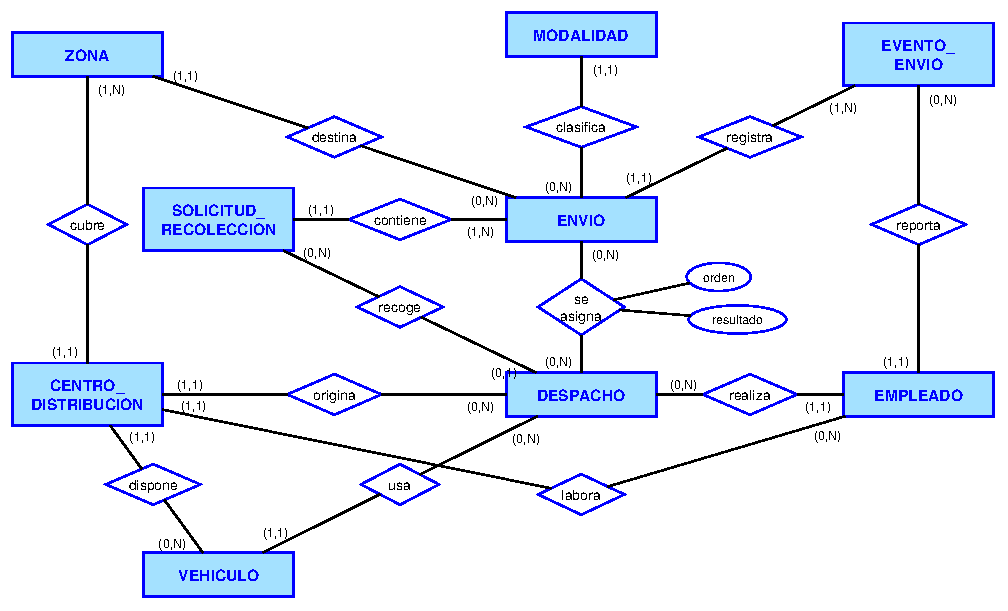
\includegraphics{figuras/er/M_U2.pdf}}
\caption{Vista U2 en el módulo: personal del centro de distribución.}
\label{fig:vistaU2}
\end{figure}
\par}

\textbf{U3 -- Mesa de servicio} (figura~\ref{fig:vistaU3}). Ve el envío
desde el cliente: quién lo pide, desde qué sede, a qué zona va, qué le
ha pasado y qué reclamaciones hay sobre él.

{\singlespacing
\begin{figure}[!htb]
\centering
\adjustbox{max width=\linewidth, max totalheight=0.42\textheight}{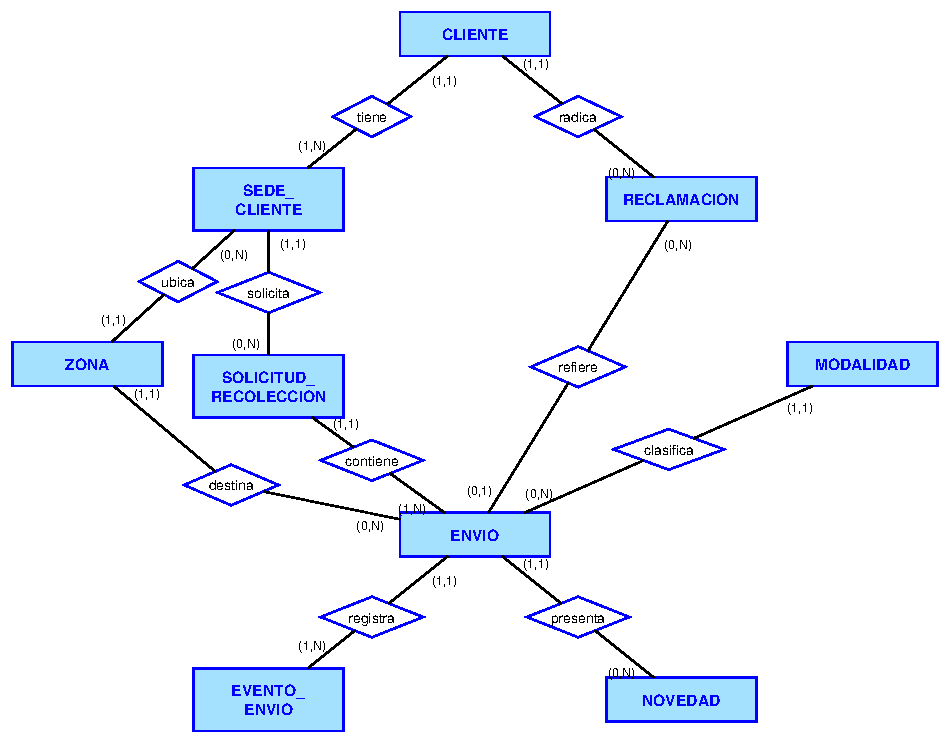
\includegraphics{figuras/er/M_U3.pdf}}
\caption{Vista U3 en el módulo: mesa de servicio.}
\label{fig:vistaU3}
\end{figure}
\par}

\textbf{U4 -- Mensajero} (figura~\ref{fig:vistaU4}). Trabaja con su
despacho del día: lo que recoge, lo que entrega y lo que registra en cada
visita (evento, prueba de entrega o novedad). Esta vista se presenta en
Data Modeler; allí la relación N:M entre ENVIO y DESPACHO
aparece como una entidad intermedia. Su versión en notación de Chen está
en la figura~\ref{fig:vistaU4chen} del anexo~\ref{anx:chen}.

{\singlespacing
\begin{figure}[!htb]
\centering
\adjustbox{max width=\linewidth, max totalheight=0.5\textheight}{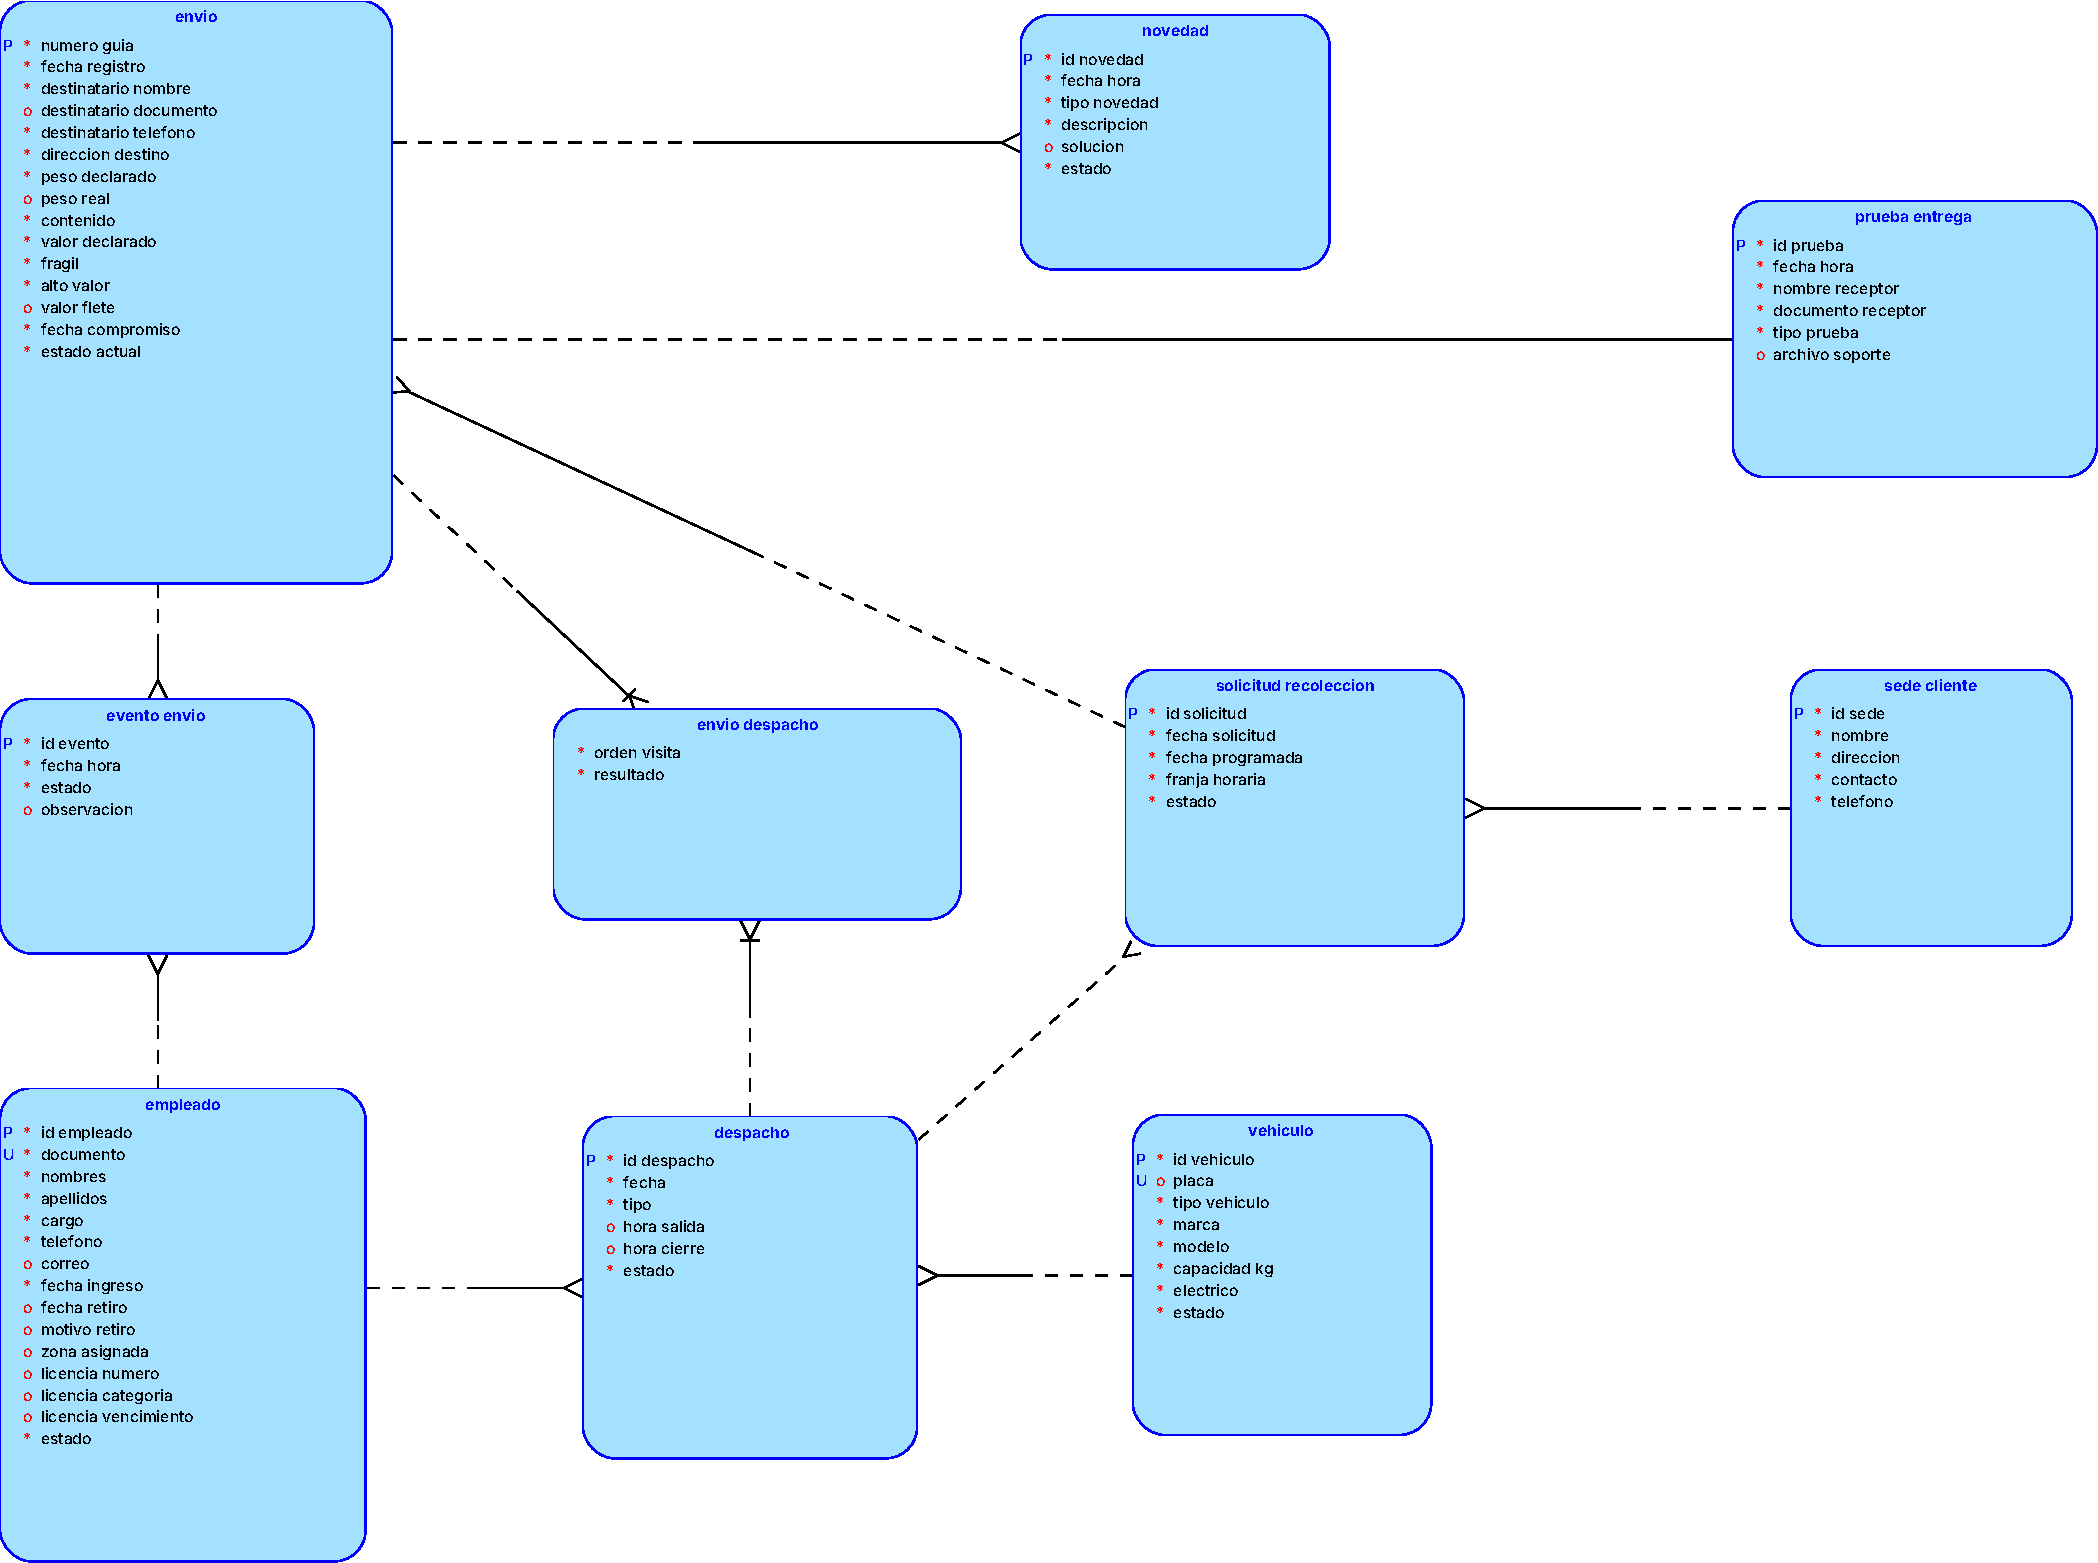
\includegraphics{figuras/datamodeler/dm_U4.pdf}}
\caption{Vista U4: mensajero, en Data Modeler (notación Barker).}
\label{fig:vistaU4}
\end{figure}
\par}

\subsubsection{Integración de Vistas (Prediseño Conceptual de la BD -- Modelo Entidad Relación)}
\label{sec:integracion}

Las vistas se integraron en cuatro pasos:

\begin{enumerate}[label=\arabic*.,leftmargin=1.2cm,itemsep=2pt]
  \item \textbf{Entidades comunes.} Las que aparecen en varias vistas
        (ENVIO, DESPACHO, ZONA, SOLICITUD\_RECOLECCION) representan lo
        mismo y quedan una sola vez; cuando una relación aparece en
        varias vistas se toma la participación más restrictiva.
  \item \textbf{Conflictos de nombre.} \textit{Guía} y \textit{paquete}
        se unifican en ENVIO; \textit{ruta} y \textit{planilla} en
        DESPACHO; \textit{conductor} y \textit{mensajero} en EMPLEADO;
        \textit{punto de recolección} en SEDE\_CLIENTE; \textit{rastreo}
        en EVENTO\_ENVIO.
  \item \textbf{Conflictos de estructura.} El estado del envío es
        atributo para la mesa de servicio y entidad (EVENTO\_ENVIO) para
        el centro; la zona fija del mensajero es atributo de EMPLEADO. El
        prediseño los deja así a propósito, como los describen los
        usuarios, y los corrige en la sección~\ref{sec:ajustes}.
  \item \textbf{Relaciones redundantes.} En el modelo global se eliminó
        la relación CLIENTE--\textit{envía}--ENVIO de la vista U7, que se
        obtiene por la sede y la solicitud (anexo~\ref{anx:global}). Entre
        las vistas del módulo no hay redundancias.
\end{enumerate}

El resultado es el prediseño del módulo (figura~\ref{fig:erintegrado}),
con 14 entidades y las 20 relaciones de la tabla~\ref{tab:relaciones}.
Es el subconjunto del prediseño global (figura~\ref{fig:erintegradoglobal})
formado por las entidades del módulo. Para compararlo con el resultado final, la
figura~\ref{fig:dmlogico} muestra a continuación el modelo del módulo
después de los ajustes de la sección~\ref{sec:ajustes}, construido en
Oracle SQL Developer Data Modeler.

\begin{landscape}
{\singlespacing
\begin{figure}[p]
\centering
\adjustbox{max width=22.5cm, max totalheight=14.6cm}{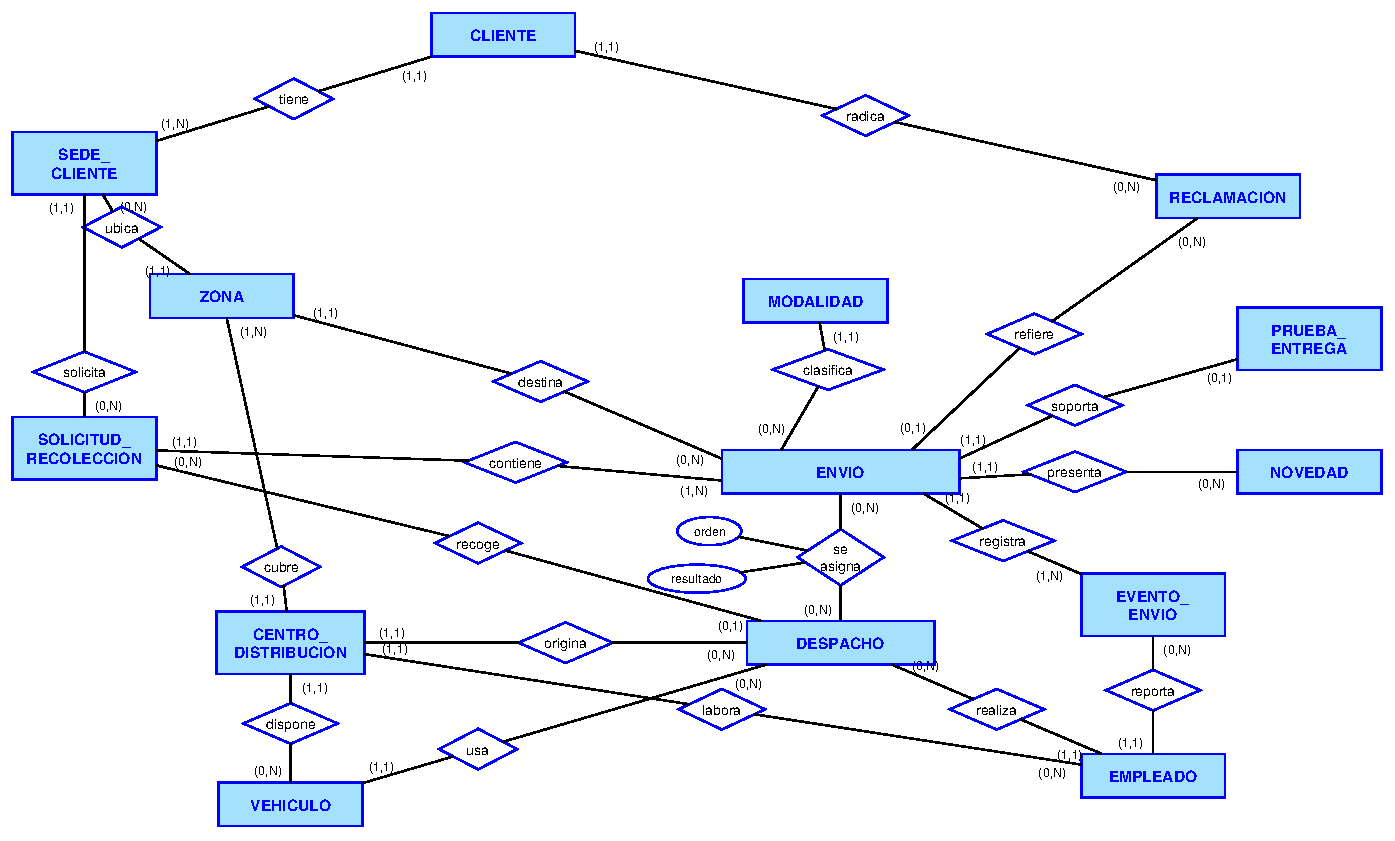
\includegraphics{figuras/er/M_prediseno.pdf}}
\caption{Prediseño conceptual del módulo de operación de envíos.}
\label{fig:erintegrado}
\end{figure}
\par}
\end{landscape}
\begin{landscape}
{\singlespacing
\begin{figure}[p]
\centering
\adjustbox{max width=22.5cm, max totalheight=14.6cm}{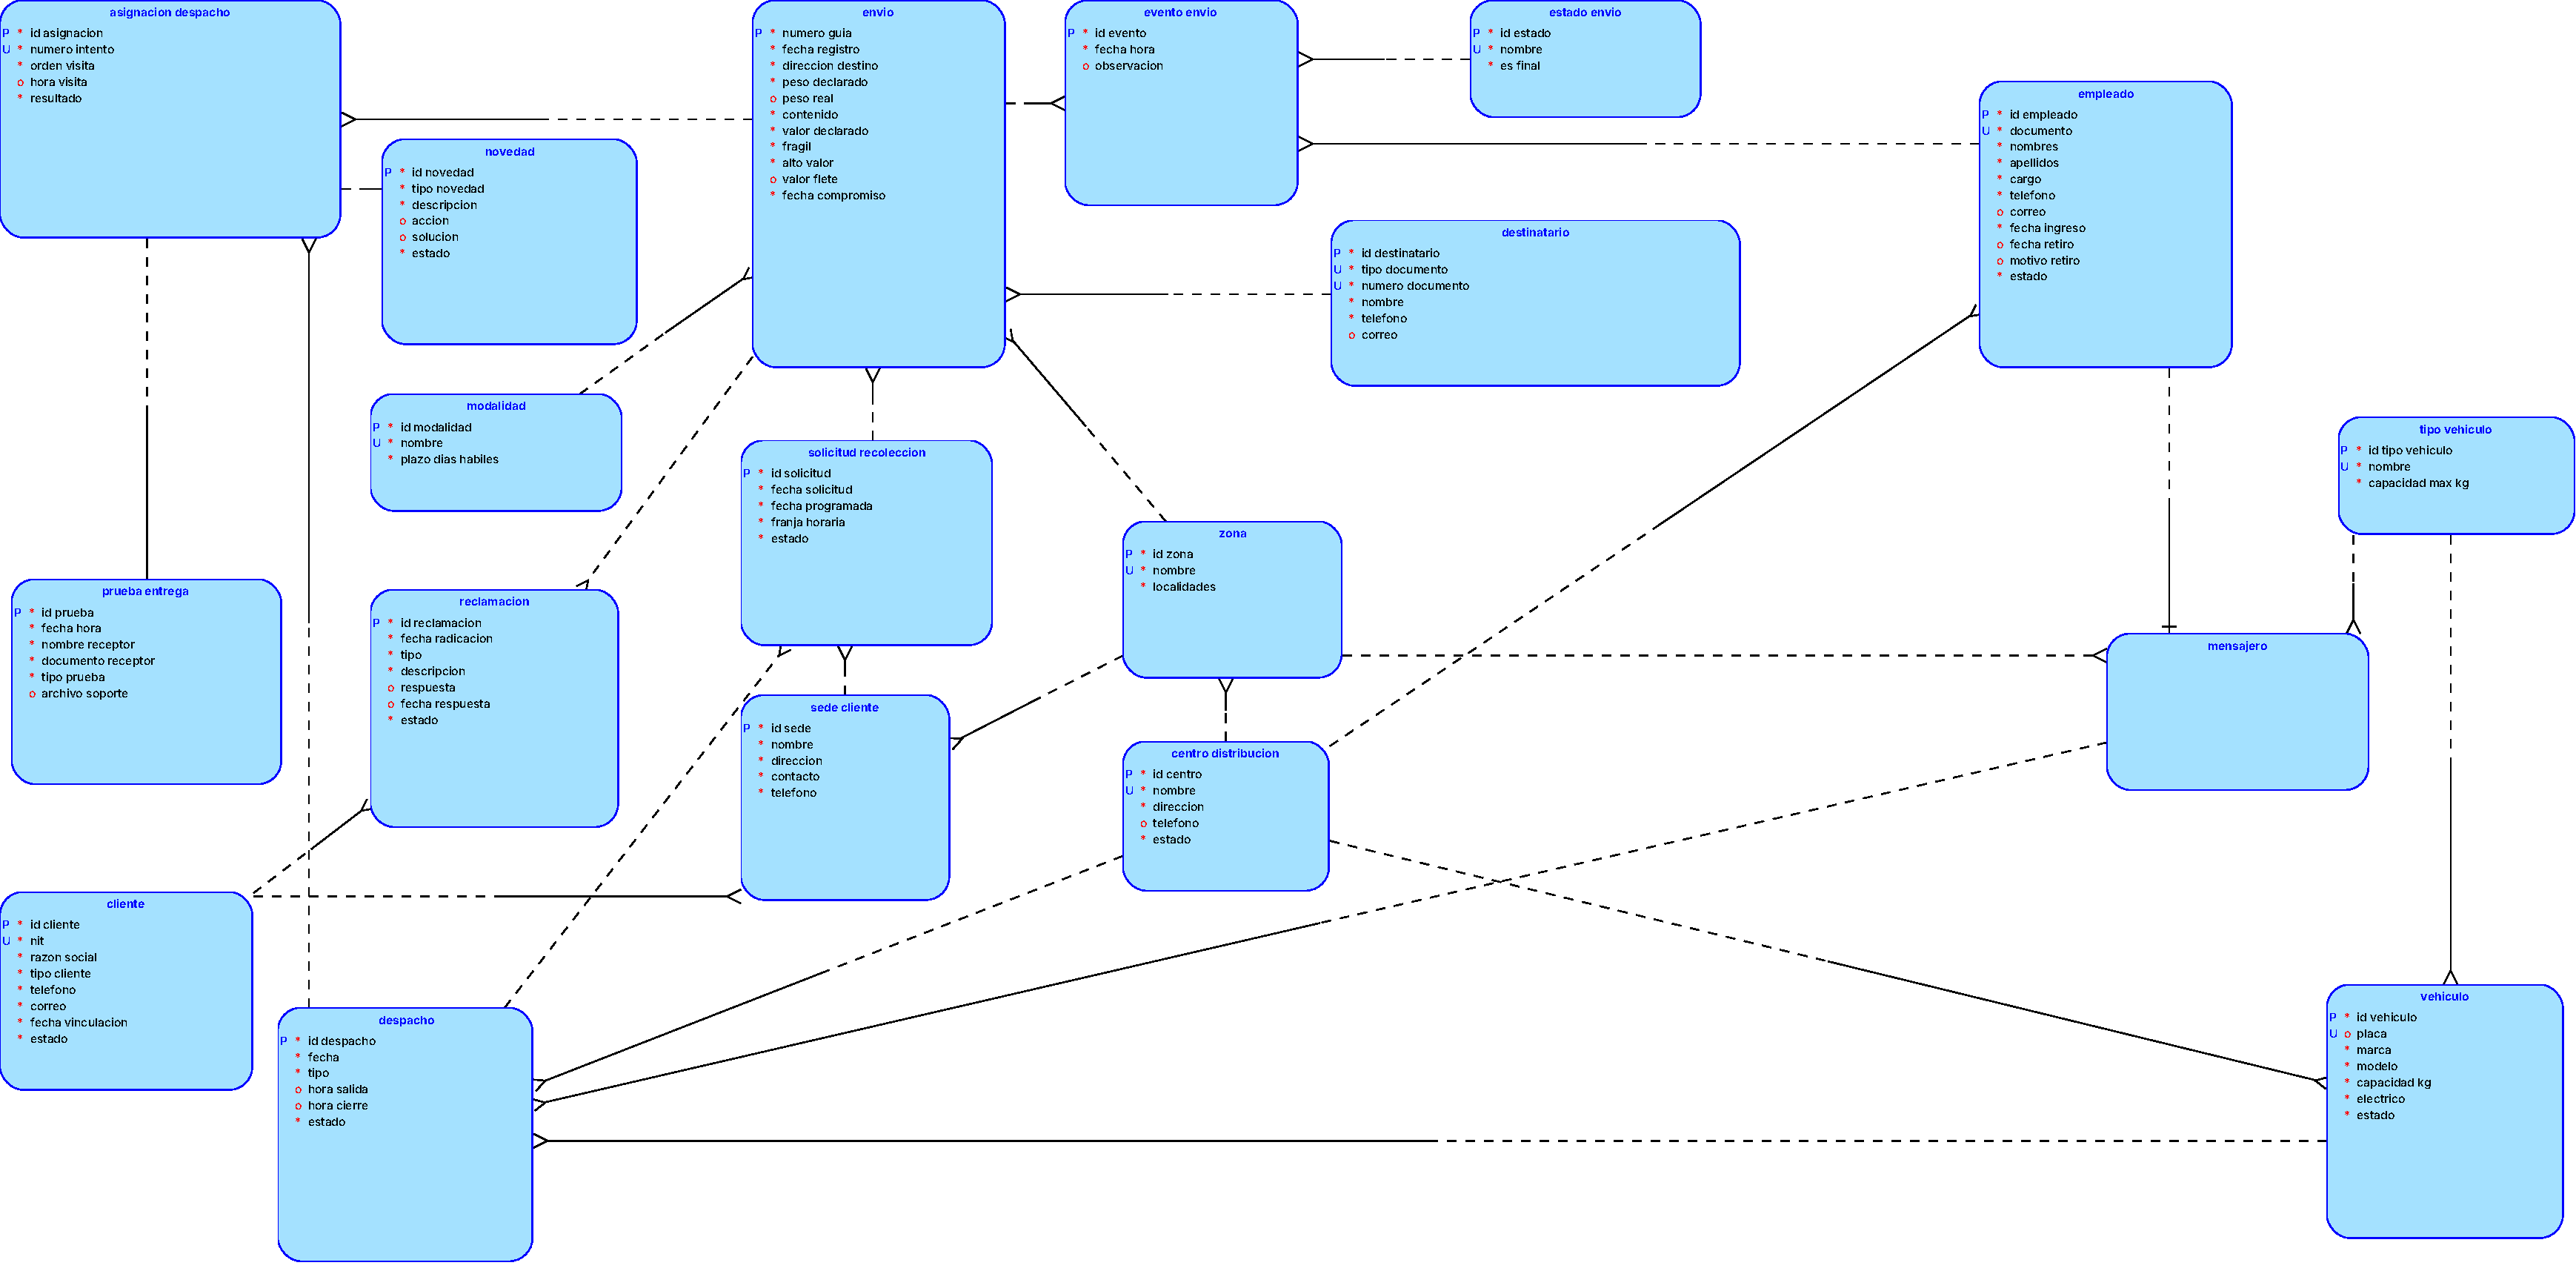
\includegraphics{figuras/datamodeler/dm_M_logico.pdf}}
\caption{Modelo Entidad-Relación ajustado del módulo de operación de envíos (resultado de los ajustes de la sección~\ref{sec:ajustes}), en Data Modeler (notación Barker).}
\label{fig:dmlogico}
\end{figure}
\par}
\end{landscape}
{\singlespacing\small
\begin{longtable}{L{1.5cm} L{4.9cm} L{0.8cm} L{2.4cm} L{3.9cm}}
\caption{Relaciones del prediseño del módulo.}
\label{tab:relaciones}\\
\toprule
\textbf{Relación} & \textbf{Entidades} & \textbf{Tipo} & \textbf{(mín,máx)} & \textbf{Significado} \\
\midrule
\endfirsthead
\toprule
\textbf{Relación} & \textbf{Entidades} & \textbf{Tipo} & \textbf{(mín,máx)} & \textbf{Significado} \\
\midrule
\endhead
\bottomrule
\endfoot
\textit{cubre} & CENTRO\_DISTRIBUCION --\allowbreak\ ZONA & 1:N & (1,1) -- (1,N) & Cada zona es atendida por un solo centro. \\
\textit{labora} & CENTRO\_DISTRIBUCION --\allowbreak\ EMPLEADO & 1:N & (1,1) -- (0,N) & Cada empleado trabaja en un centro. \\
\textit{dispone} & CENTRO\_DISTRIBUCION --\allowbreak\ VEHICULO & 1:N & (1,1) -- (0,N) & Cada vehículo está asignado a un centro. \\
\textit{origina} & CENTRO\_DISTRIBUCION --\allowbreak\ DESPACHO & 1:N & (1,1) -- (0,N) & Cada despacho sale de un centro. \\
\textit{ubica} & ZONA --\allowbreak\ SEDE\_CLIENTE & 1:N & (1,1) -- (0,N) & Cada sede del cliente está en una zona. \\
\textit{destina} & ZONA --\allowbreak\ ENVIO & 1:N & (1,1) -- (0,N) & Zona a la que va cada envío. \\
\textit{tiene} & CLIENTE --\allowbreak\ SEDE\_CLIENTE & 1:N & (1,1) -- (1,N) & Sedes de recolección de cada cliente. \\
\textit{clasifica} & MODALIDAD --\allowbreak\ ENVIO & 1:N & (1,1) -- (0,N) & Modalidad contratada para cada envío. \\
\textit{solicita} & SEDE\_CLIENTE --\allowbreak\ SOLICITUD\_RECOLECCION & 1:N & (1,1) -- (0,N) & Solicitudes hechas desde cada sede. \\
\textit{contiene} & SOLICITUD\_RECOLECCION --\allowbreak\ ENVIO & 1:N & (1,1) -- (1,N) & Envíos que se recogen en cada solicitud. \\
\textit{recoge} & DESPACHO --\allowbreak\ SOLICITUD\_RECOLECCION & 1:N & (0,1) -- (0,N) & Despacho de recolección que atiende cada solicitud. \\
\textit{se asigna} & ENVIO --\allowbreak\ DESPACHO & N:M & (0,N) -- (0,N) & Un envío puede salir en varios despachos (reintentos) y un despacho lleva muchos envíos. Atributos: orden, resultado. \\
\textit{registra} & ENVIO --\allowbreak\ EVENTO\_ENVIO & 1:N & (1,1) -- (1,N) & Historial de estados de cada envío. \\
\textit{reporta} & EMPLEADO --\allowbreak\ EVENTO\_ENVIO & 1:N & (1,1) -- (0,N) & Empleado responsable de cada evento. \\
\textit{soporta} & ENVIO --\allowbreak\ PRUEBA\_ENTREGA & 1:1 & (1,1) -- (0,1) & Constancia de recibo de cada envío. \\
\textit{presenta} & ENVIO --\allowbreak\ NOVEDAD & 1:N & (1,1) -- (0,N) & Novedades ocurridas con cada envío. \\
\textit{radica} & CLIENTE --\allowbreak\ RECLAMACION & 1:N & (1,1) -- (0,N) & Reclamaciones hechas por cada cliente. \\
\textit{refiere} & ENVIO --\allowbreak\ RECLAMACION & 1:N & (0,1) -- (0,N) & Envío sobre el que trata una reclamación (opcional). \\
\textit{usa} & VEHICULO --\allowbreak\ DESPACHO & 1:N & (1,1) -- (0,N) & Vehículo con el que se hace cada despacho. \\
\textit{realiza} & EMPLEADO --\allowbreak\ DESPACHO & 1:N & (1,1) -- (0,N) & Empleado (mensajero) que hace cada despacho. \\
\end{longtable}
\par}

%-----------------------------------------------------------------------
\subsection{Determinación de requerimientos de procesamiento}

Los requerimientos de procesamiento indican qué entra a la base de
datos, qué se hace con ello y qué se obtiene; de aquí salen las vistas,
consultas y procedimientos de los capítulos 4 a 6.

\subsubsection{Determinación de entradas, procesos y salidas por usuario}
\label{sec:eps}

La tabla~\ref{tab:eps} presenta los usuarios del módulo; los de los
demás módulos están en el anexo~\ref{anx:analisis}
(tabla~\ref{tab:epsotros}).

{\singlespacing\small
\begin{longtable}{L{1.9cm} L{3.9cm} L{4.6cm} L{3.9cm}}
\caption{Entradas, procesos y salidas de los usuarios del módulo.}
\label{tab:eps}\\
\toprule
\textbf{Usuario} & \textbf{Entradas} & \textbf{Procesos} & \textbf{Salidas} \\
\midrule
\endfirsthead
\toprule
\textbf{Usuario} & \textbf{Entradas} & \textbf{Procesos} & \textbf{Salidas} \\
\midrule
\endhead
\bottomrule
\endfoot
U1 Gerente general &
Periodo, centro o zona a consultar. &
Calcular el porcentaje de entregas a tiempo, el de envíos con novedad y
el tiempo de respuesta a reclamaciones. (Los indicadores de facturas,
rotación y flota se agregan con los demás módulos.) &
Indicadores de operación frente a las metas de la
tabla~\ref{tab:metas}. \\
\midrule
U2 Personal del centro &
Centros y zonas; programación de recolecciones; peso real de cada
paquete; valor del flete; envíos, mensajero y vehículo de cada despacho;
hora de salida y de cierre. &
Validar que el vehículo esté disponible y el mensajero activo antes de
crear el despacho (la validación de documentos, licencia y capacitación
se completa con M3 y M4); registrar eventos \textit{Recolectado},
\textit{En centro}, \textit{Clasificado} y \textit{En ruta}. &
Planilla de despacho; envíos pendientes por zona y modalidad; envíos que
vencen hoy; resultado del cierre de ruta. \\
\midrule
U3 Mesa de servicio &
Solicitudes de recolección; datos de los envíos y destinatarios;
decisiones sobre novedades; reclamaciones y sus respuestas. &
Verificar que el cliente esté activo (el contrato vigente se valida con
M2); generar el número de guía; controlar el número de intentos de
entrega; calcular el tiempo de respuesta de cada reclamación. &
Guía del envío; recorrido de un envío; novedades abiertas; reclamaciones
pendientes. \\
\midrule
U4 Mensajero &
Confirmación de recolección; prueba de entrega (firma, documento o
fotografía); novedad con su tipo. &
Registrar el evento con la fecha, la hora y el mensajero; impedir marcar
como entregado un envío sin prueba; impedir entregar a terceros los
envíos frágiles o de alto valor. &
Lista de su despacho con el orden de visita; datos de contacto del
destinatario. \\
\midrule
U9 Cliente &
Número de guía. &
Verificar que la guía pertenezca al cliente que consulta. &
Estado actual y recorrido del envío. \\
\end{longtable}
\par}

%-----------------------------------------------------------------------
\subsection{Ajustes al Diseño Conceptual de la BD -- Modelo Entidad Relación}
\label{sec:ajustes}

Al revisar el prediseño contra los requerimientos de procesamiento se
hicieron los ajustes de la tabla~\ref{tab:ajustes}. Los ajustes 1 a 5
se aplicaron al modelo global (anexo~\ref{anx:global}); el 6 es propio
del módulo.

{\singlespacing\small
\begin{longtable}{L{0.8cm} L{3.9cm} L{4.6cm} L{5.1cm}}
\caption{Ajustes realizados al prediseño conceptual.}
\label{tab:ajustes}\\
\toprule
\textbf{N.º} & \textbf{En el prediseño} & \textbf{Ajuste} & \textbf{Justificación} \\
\midrule
\endfirsthead
\toprule
\textbf{N.º} & \textbf{En el prediseño} & \textbf{Ajuste} & \textbf{Justificación} \\
\midrule
\endhead
\bottomrule
\endfoot
1 &
Los datos del destinatario (nombre, documento, teléfono) son atributos
de ENVIO. &
Se crea la entidad DESTINATARIO, relacionada con ENVIO mediante
\textit{dirigido} (1:N). La dirección de entrega y la zona se mantienen
en ENVIO. &
Las droguerías y tiendas envían con frecuencia a las mismas personas, lo
que repetía sus datos en cada envío. Además, la Ley 1581 exige poder
consultar, corregir o suprimir los datos de una persona, lo que es más
sencillo si están en un solo registro. La dirección se deja en el envío
porque puede cambiar de un envío a otro. \\
\midrule
2 &
La relación ENVIO--\textit{se asigna}--DESPACHO es N:M, con los
atributos orden y resultado. PRUEBA\_ENTREGA y NOVEDAD se relacionan
directamente con ENVIO. &
La relación se convierte en la entidad ASIGNACION\_DESPACHO, que
representa cada intento de entrega o recolección de un envío en un
despacho. PRUEBA\_ENTREGA y NOVEDAD pasan a relacionarse con ella
(1:1). &
Un envío puede salir en varios despachos (reintentos y devolución) y
cada intento termina en una entrega o en una novedad. Con el cambio se
sabe en qué intento, con qué mensajero y en qué despacho ocurrió cada
novedad, y se puede controlar el máximo de dos intentos. \\
\midrule
3 &
EMPLEADO tiene como atributos la zona asignada y los datos de la
licencia, aunque solo aplican a los mensajeros. EMPLEADO realiza
DESPACHO. &
Se crea MENSAJERO como especialización de EMPLEADO. La zona pasa a ser
la relación ZONA--\textit{atiende}--MENSAJERO, la licencia pasa a la
entidad LICENCIA\_CONDUCCION (1:N) y el despacho lo realiza un
MENSAJERO. En el módulo no se incluye LICENCIA\_CONDUCCION, que
pertenece a M4. &
Evita atributos vacíos para el resto de empleados, garantiza que solo un
mensajero pueda recibir un despacho y conserva el historial de licencias
(renovaciones y categorías), necesario para validar la vigencia en la
fecha del despacho. \\
\midrule
4 &
EVENTO\_ENVIO tiene el estado como texto libre y ENVIO guarda además el
estado actual. &
Se crea el catálogo ESTADO\_ENVIO, relacionado con EVENTO\_ENVIO
(\textit{indica}, 1:N). El estado actual se retira de ENVIO porque se
obtiene del último evento. &
Los indicadores y las reglas dependen de estados escritos siempre igual.
Guardar el estado en dos lugares permite que se contradigan; si en el
diseño físico se requiere por rendimiento, se agregará como dato
derivado controlado por la base de datos. \\
\midrule
5 &
El tipo de vehículo y el tipo de documento son atributos de texto de
VEHICULO y DOCUMENTO\_VEHICULO. &
Se crean los catálogos TIPO\_VEHICULO y TIPO\_DOCUMENTO, con la relación
\textit{exige} (N:M) entre ellos. El módulo solo incorpora
TIPO\_VEHICULO, porque VEHICULO lo referencia; lo demás es de M3. &
La política de seguridad vial exige que ningún documento
\textit{obligatorio} esté vencido. Con solo las fechas no se detecta un
documento que nunca se registró; con \textit{exige} se sabe qué
documentos debe tener cada tipo de vehículo (por ejemplo, la bicicleta
eléctrica no requiere SOAT). \\
\midrule
6 &
MENSAJERO guarda como texto el tipo de vehículo que puede conducir. &
Se reemplaza por la relación TIPO\_VEHICULO--\textit{conduce}--MENSAJERO
(1:N). Aplica solo al módulo. &
Evita escribir el mismo tipo de varias formas y permite verificar que
el vehículo de un despacho sea del tipo que conduce su mensajero. \\
\end{longtable}
\par}

El modelo ajustado del módulo tiene 19 entidades y 26 relaciones, más
la especialización parcial de EMPLEADO en MENSAJERO (no todos los
empleados son mensajeros). Se presenta en la figura~\ref{fig:dmlogico},
a continuación del prediseño; el diagrama en notación de Chen, con el
nombre de cada relación y su participación (mín,máx), está en la
figura~\ref{fig:erfinal} del anexo~\ref{anx:chen}. Ambos diagramas se
verificaron relación por relación; el de Data Modeler muestra 27
relaciones y no 26 porque la especialización EMPLEADO--MENSAJERO aparece
como una relación 1:1 identificadora. Respecto al
prediseño, se agregan DESTINATARIO, ASIGNACION\_DESPACHO, ESTADO\_ENVIO,
MENSAJERO y TIPO\_VEHICULO, y la relación N:M \textit{se asigna} se
reemplaza por ASIGNACION\_DESPACHO. Sus atributos se definen en el
diccionario de datos (sección~\ref{sec:diccionario}). Este modelo es la
entrada del diseño lógico.

